\section{Discussion}
\label{sec:discussion}

As can be seen, our approach only provides a noticeable improvement to the performance of Cassandra when multiple nodes in the cluster are heavily loaded. This is not what we initially imagined our results would be. One of our intuitions is that the performance decrease exists because the resource usage formula does not accurately reflect what the time to execute a query will be. To confirm this intuition we performed an experiment that compared the resource usage to the query execution time in a Cassandra instance.

In the remainder of this section we will provide what we feel will be a more accurate resource usage formula for distributed databases, as well as discuss several limitations that may also have affected our work.

\subsection{Re-examining the Resource Usage formula}
\label{sec:examineResUse}

\begin{figure}[t]
\centering
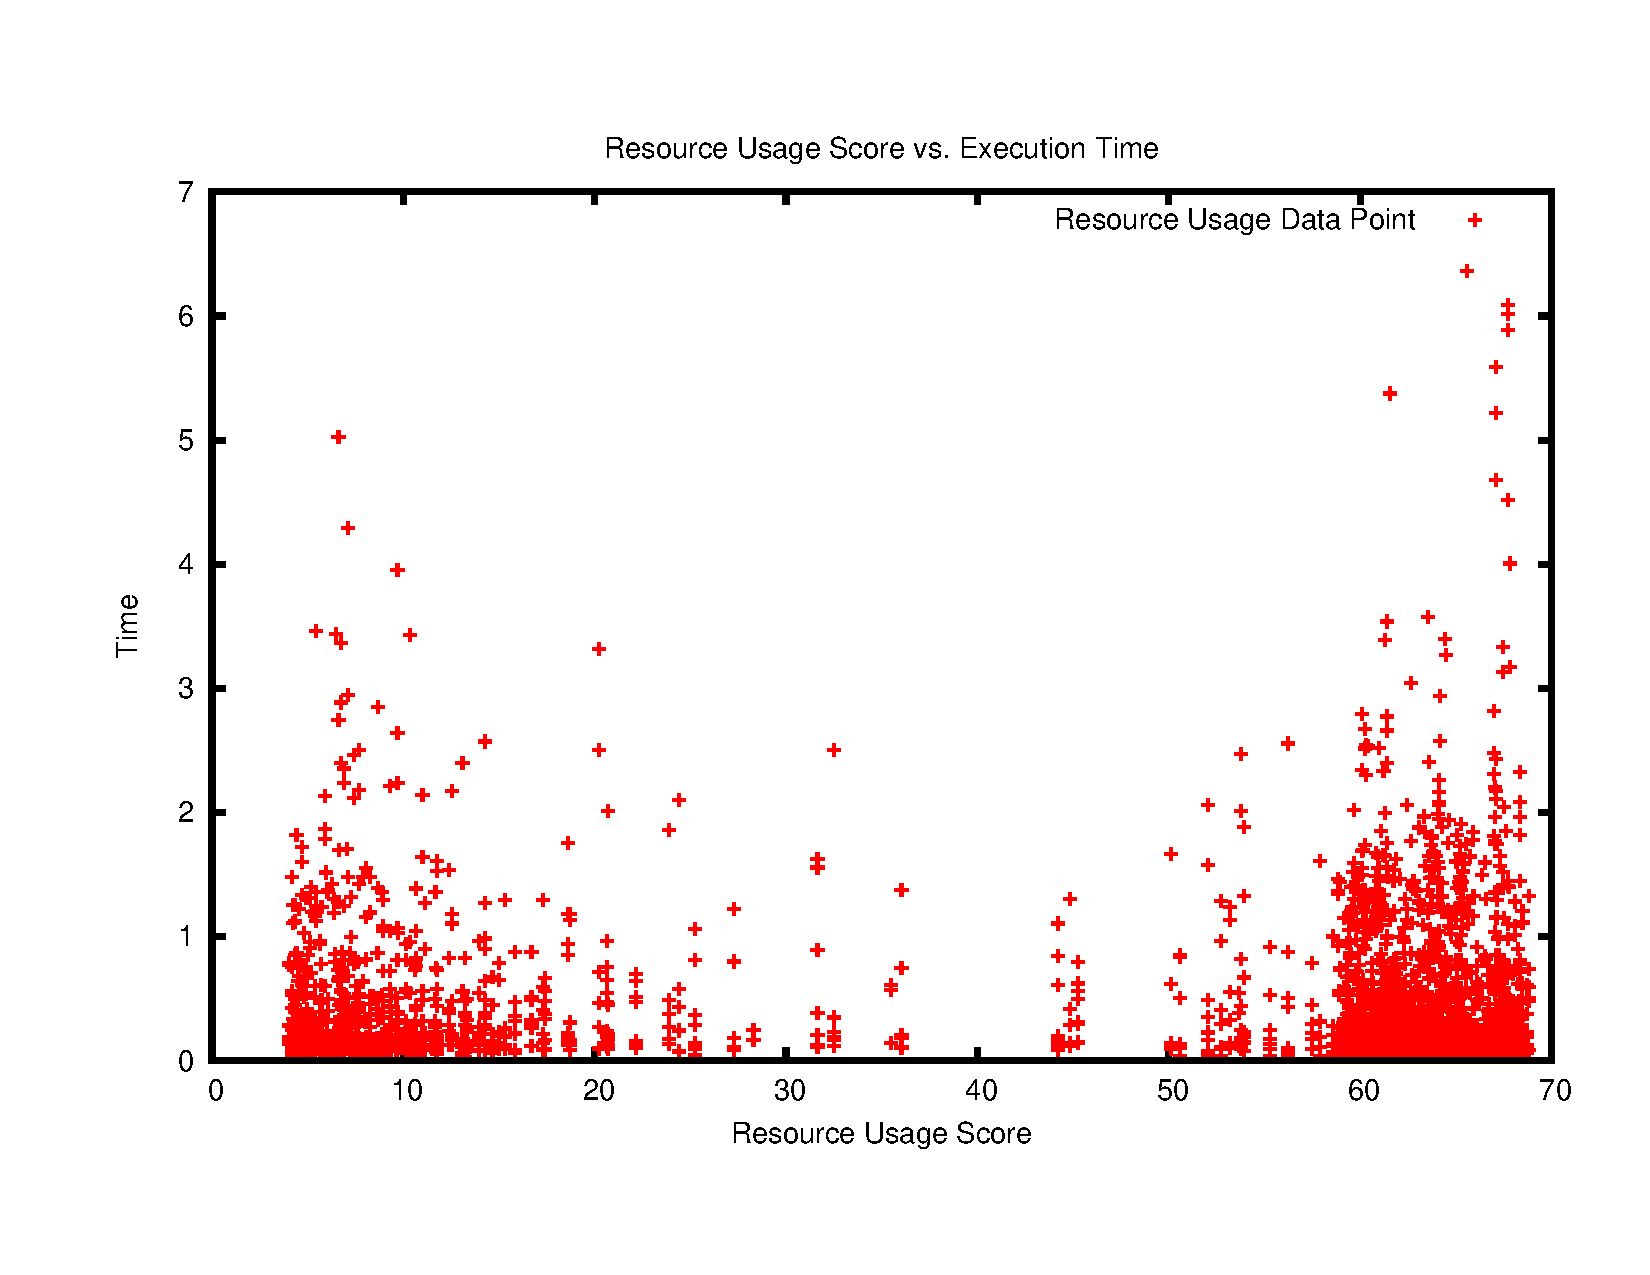
\includegraphics[scale=0.3]{images/ResUse.pdf}
\vspace{-15pt}
\caption{The experimental results comparing the resource usage score to the query execution time.}
\label{fig:resourceUsageFig}
\end{figure}

To examine how representative the resource usage score is we have performed an experiment that compares resource usage to query execution time. The setup for the resource usage experiments is different than the setup for the primary experiments. This experiment was performed on a single Cassandra instance on a single machine with a 4-core 2.6Ghz processor and 8GB of memory. The server also contained a solid-state drive instead of the hard disk drive used in the servers in the cluster. The settings for YCSB and Cassandra were identical, except that the replication factor was set to \textit{one}.

The CPU usage and memory usage was recorded every 250ms, and the query execution time was recorded for each query. The queries that executed in that 250ms window had their execution time averaged. The CPU usage and memory usage were used to calculate the resource usage of the server for each 250ms interval. The results were gathered over a 300 second interval using 10 parallel YCSB clients. Given our previous results showing that even 1000 parallel clients did not heavily load the node servers we do not believe that the results would be any different for a number of parallel clients greater than 10.

The results from the experiment are shown in Figure~\ref{fig:resourceUsageFig}. There appears to be little correlation between the resource usage score and the query execution time. When the resource usage score is higher, there are slightly more outliers that require a longer execution time, but in most cases the execution time seems to be independent of the resource usage. In addition, the resource usage scores tend to either be very low or very high. While this experiment was running, we also periodically loaded the server with other work. This resulted in a higher resource usage score, but not in a higher query execution time.

This experiment seems to indicate that the current formula is not ideal for determining the resource usage of the server. However, we believe that this could still work if the formula was changed to reflect how some variables affect the query execution time much more.  Additional variables can also be added that affect query execution time. For example, one of the primary bottlenecks in any database system is the hard disk, and we do not consider any variables related to the disk (e.g., disk access throughput).

Something to note is that the heap memory of the Cassandra instance rarely exceeded 1GB. Meaning that the memory usage score had little effect during the normal experiments. Even when the server was being artificially loaded the heap memory therefore has little effect. This also means that little data is being cached, which increases the importance of measuring the disk load.

\subsection{The New Resource Usage Formula}
\label{sec:usageFormula}
As Section~\ref{sec:examineResUse} shows, the resource usage score is far from ideal. We have some ideas on how to create a better resource usage formula. For reference, the current resource usage formula is:

\begin{center}
$ResourceUsage = \frac{1}{1-CPU} \times \frac{1}{1-Memory}$
\end{center}

The new resource usage formula is:
\begin{center}
$ResourceUsage = \frac{1}{1-CPU} \times j\left ( \frac{1}{1-Memory} \right ) \times k\left ( \frac{1}{1-Disk} \right ) \times \frac{1}{1-Distance}$
\end{center}

This is our proposed new equation that we feel may be more representative of the machine condition and should work better as a reference for assigning jobs. As can be seen, the \textit{CPU usage} and \textit{Memory usage} are still in the equation. We have added parameters for \textit{Disk} usage, \textit{Distance} (network overhead) and two scaling parameters:

\begin{itemize}
\item{\textit{Disk}} \\
\textit{Disk} refers to the hard disk performance of the machine. We feel this value should be related to values such as the average disk access time and data transfer rate. It will also be related to the disk usage condition by all programs on the machine. The slower the disk is by nature, and the busier the disk is being used by the programs, the higher the value of \textit{Disk} will be. 
\item{Distance} \\
\textit{Distance} is referring to the distance between the node servers and the network conditions. This value will be determined by both the physical network ability, like the total available bandwidth; and the network conditions, like current network usage. This parameter is very important in affecting affect the execution time when dealing with multiple datacenters.
\item{Parameters \textit{k,j}} \\
The different server performance parameters have a different magnitude of effect on the query execution time. For example, from what we observed during the experiments, memory usage has little influence on the query execution time while \textit{disk usage} affects the execution time a lot. This importance level is adjusted by the constant coefficients \textit{j} and \textit{k} in the equations. \textit{Memory} is less important so \textit{j} should probably be less than 1 and \textit{disk} is very important so \textit{k} is probably bigger than 1. The exact value of these parameters would need to be determined with further testing.
\end{itemize}

This equation is just a representation of our idea and isn't necessarily accurate. More experiments are needed to confirm that this equation leads to better performance. 

\subsection{Limitations}
Our system only provides better performance in very limited cases. Apart from the reasons listed in Section~\ref{sec:experiments} we believe that our experiment is limited due to the following reasons:

\paragraph{Limited test environment}
As mentioned earlier, we only have ten servers in our experiment which limits the replica allocation. The distance between the servers is also extremely short, such that latency was never as issue. In reality, there are an average of 100,000 servers in a data center~\cite{Guo:2010:SDC:1921168.1921188}, and replication and backup processes may occur between data centers~\cite{F5-Accelerate}. In addition, normally every one mile in distance will add 8.2 microseconds latency to the performance, and this number does not consider package drop, switch delay, and link size~\cite{Cisco-Latency}. This implies that one mile in distance between servers will have a delay greater than 8.2 microseconds. Replication between datacenters and a large amount of servers will result in longer distance communication, and this is, we believe, the distance between servers is also a very important factor while performing workload partitioning.
 
\paragraph{Simplistic workload}
The queries, which we use for testing our system, are too simple. Even though we implement our algorithm on the most time consuming queries in Cassandra the CPU and memory consumption is still rare. This is because we are using a key-value database where the operations are fairly simple and multiple optimizations have already been implemented. This seems to partially account for why our approach does not introduce any performance improvement to the original query assignment system.
 
\paragraph{Unable to congest the network manually}
Network congestion occurs when a link is carrying so much data that is greater than the capacity of the network. This causes queuing delay, packet loss, and a high chance of failure~\cite{103559}. However, we do not have this issue in our experiment, because our severs are located in close proximity and the network is never congested. This eliminates the chance to test our system under this situation.
 
\paragraph{Disk information was not considered}
Many researchers point out that the hard disk drive access times are lagging behind processor improvements, and consequently, the performance gap between processors and hard disk drives is increasing. This results in I/O wait time increasing as a percentage of processor utilization. As result, disk bottlenecks occur~\cite{IBM-IO, TMS-SSD}. This problem can partially solved by using a large amount of main memory, so as to avoid disk access for intermediate results; however main memory is not free and infinite. When there are large amount of multi-query workloads are trying to perform I/O operation, the memory will be filled up and disk bottlenecks~\cite{Bouganim:1998:MSL:288627.288646} will occur. This indicates that the disk seek time is crucial. However, our experiment only examined CPU time, which is always fast and does not have a very significant impact on the query execution time.

\subsection{Future Work}
As mentioned above, we want to validate our proposed new resource usage formula (see Section~\ref{sec:usageFormula}) by running experiments on it. After determining a more accurate representation for the resource usage of a machine, the experiments could be redone to see if it leads to better performance. At the same time, we should continue to reduce the overhead of the query assignment algorithm as overhead is one of the key factors that affect the performance of the database.

We would also like to test our new algorithm on other key-value databases (e.g., HBase) and other types of databases (e.g., distributed relational databases). In the case of relational databases, more complex queries could be used to see how the complexity of queries affect the performance.

\section{Conclusion}
\label{sec:conclusion}

Because the code that handles scans is completely disjoint from the code that handles reads, writes or updates it is plausible to implement our algorithm purely for scans while losing very little performance (just the overhead of a single thread in Cassandra that queries the CJD for resource information).
